%%%%%%%%%%%%%%%%%%%%%%%%%%%%%%%%%%%%%%%%%
% Beamer Presentation
% LaTeX Template
% Note:
% data cleaning should be added
% https://realpython.com/python-data-cleaning-numpy-pandas/
% 


\documentclass{beamer}
\mode<presentation> {
\usetheme{Warsaw}
}

\usepackage{multicol}
\usepackage[russian]{babel}
\usepackage{graphicx} 
\usepackage{hyperref}

\title[Introduction to Python]{SQL with Python} 
\author{Sugarkhuu Radnaa} 
\institute[]
{
Py4Econ in Ulaanbaatar \\ 
\medskip
\textit{py4econ@gmail.com} 
}
\date{}  %15 January, 2022 \today

\begin{document}

\begin{frame}
\titlepage % Print the title page as the first slide
\end{frame}

\begin{frame}
    \frametitle{Week 4: Learning objectives}
    Get to know: 
    \begin{enumerate}
        \item Basic concepts about SQL and structured database
        \item PostgreSQL and PgAdmin
        \item Using PostgreSQL in terminal
        \item Working with SQL using Python
    \end{enumerate}
\end{frame}

%------------------------------------------------
\section{Data types and structures} 
%------------------------------------------------

\begin{frame}
    \frametitle{SQL}
    SQL is the most popular database language. There are many different DBMS (database management system)s including structured and NoSQL. \\
    \textbf{Popular structured/SQL databases}:
    \begin{enumerate}
        \item Oracle SQL
        \item Microsoft SQL
        \item MySQL
        \item PostgreSQL
        \item SQLite
    \end{enumerate}    

    \textbf{Popular NoSQL databases}:
    \begin{enumerate}
        \item MongoDB
        \item ElasticSearch
        \item Casandra
    \end{enumerate}    
\end{frame}

\begin{frame}
    \centering
    \frametitle{Sample structured database design}
    \begin{flushleft}
        Data architecture is a crucial in any organization. When due implemented, it can become a game changing factor. Efficient ETL, Datawarehouse and 
        data centers are necessary for an efficient DBMS.        
    \end{flushleft}
    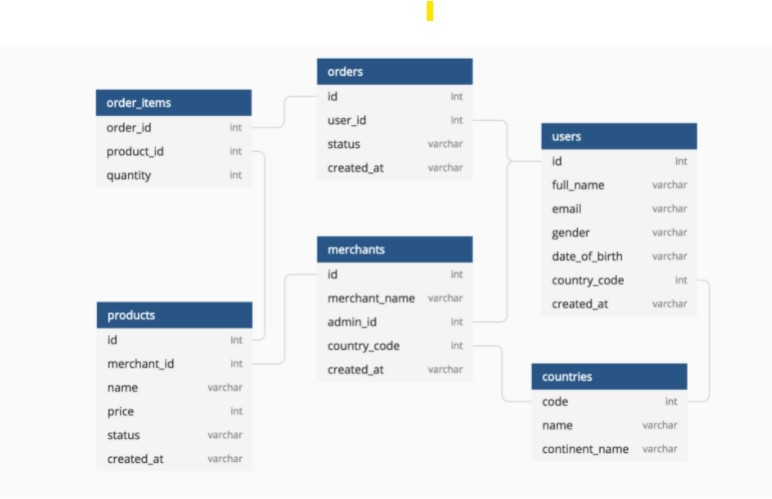
\includegraphics[scale=0.5]{figures/db_design.jpg}
\end{frame}

\begin{frame}
    \frametitle{SQL: W3SCHOOL examples}
    \begin{enumerate}
\tiny        \item SELECT CustomerName, City FROM Customers; 
        \item SELECT * FROM Customers
        WHERE Country='Mexico';
        \item SELECT * FROM Customers
        WHERE Country='Germany' AND (City='Berlin' OR City='Frankfurt');
        \item UPDATE Customers
        SET ContactName = 'Alfred Schmidt', City= 'Frankfurt'
        WHERE CustomerID = 1;
        \item SELECT * FROM Customers
        WHERE ContactName LIKE 'a\%';
        \item SELECT Customers.CustomerName, Orders.OrderID
        FROM Customers
        LEFT JOIN Orders ON Customers.CustomerID = Orders.CustomerID
        ORDER BY Customers.CustomerName;
        \item SELECT COUNT(CustomerID), Country
        FROM Customers
        GROUP BY Country
        ORDER BY COUNT(CustomerID) DESC;
    \end{enumerate}
\end{frame}

\begin{frame}
    \frametitle{Some useful tips}
    \begin{enumerate}
        \item Dump database to a file / Restore database from a file
        \item SQLite is perhaps quickest and lightest DBMS 
        \item Run routine tasks in function/procedure
    \end{enumerate}
\end{frame}

\begin{frame}
    \frametitle{psql basic terminal commands}
    \begin{enumerate}
        \item psql -U username - connect to a psql server with username
        \item \textbackslash l - list of databases 
        \item \textbackslash c dbname - choose database
        \item \textbackslash dt - list of tables in the chosen database 
        \item \textit{Command}; - Command to run (Note: a statement must be terminated with semicolon ;)
        \item \textbackslash q - quit psql
        \item pg_dump -U username -d database_name -t table_name > table_dump.sql

    \end{enumerate}
\end{frame}

%------------------------------------------------
\section{Homework} 
%------------------------------------------------

\begin{frame}
    \frametitle{Homework}
    \begin{enumerate}
        \item Task 1
    \end{enumerate}

    \vskip 2mm
    \begin{itemize}
        \item Push your result into your homework repository
        \item Deadline: 1 week %22 January, 2022
    \end{itemize}

\vfill
\textbf{Note:} Commit your results step by step.
\end{frame}

\begin{frame}
    \frametitle{Task 1}
    \begin{enumerate}
        \item Populate a PostgreSQL table with the data in “data.xlsx” (CREATE TABLE)
        \item Select 'firstName' and 'lastName' of the first three rows  ('LIMIT')
        \item Select 'firstName' and 'age' of the last three rows ('ORDER BY, LIMIT')
    \end{enumerate}
\vfill
\textbf{Tip:} Watch the following tutorial for PostgreSQL
\begin{itemize}
    \item \href{https://www.youtube.com/watch?v=xaWlS9HtWYw}{PostgreSQL}
\end{itemize}
\end{frame}

\begin{frame}
\Huge{\centerline{Thank you!}}
\end{frame}

%----------------------------------------------------------------------------------------

\end{document} 